\documentclass[a4paper,kulak]{kulakarticle} %options: kul or kulak (default)

\usepackage[utf8]{inputenc}
\usepackage[dutch]{babel}
\usepackage{wrapfig}
\usepackage{graphicx}
\usepackage{subcaption}
\usepackage{float}
\usepackage[gen]{eurosym}
\usepackage{amsmath}
\date{Academiejaar 2018 -- 2019}
\address{
  Informatica \\
  Statistische modellen en data-analyse \\
  Prof. Van Aelst, Stijn Rebry}
\title{Opdracht 2}
\author{Thomas Bamelis, Michiel Jonckheere}


\begin{document}

\maketitle

\section*{Inleiding}
In dit verslag analyseren we de gegevens van airbnb gemeten in 2019 van de steden Antwerpen, Brussel en Gent van 11.000 verblijven.
We analyseren de prijs in functie van het type, de stad en de buurt van het bedrijf.
Daarna proberen we een regressiemodel op te stellen voor de huurprijs en dit model te evalueren en te interpreteren.
Als laatste passen we logistische regressie toe om te voorspellen of een verblijf al dan niet wordt vast verhuurd in plaats van enkel voor korte periodes.\\
\textit{Opmerking:} als in dit verslag een p-waarde als nagenoeg 0 wordt beschreven, betekent dit dat de p-waarde voor underflow zorgde in het computersysteem (< 2.2e-16).
Indien het significantieniveau niet vermeld staat wordt 0.05 gehanteerd. \\
De volgende gegevens zijn beschikbaar: id, naam, uitbater id, naam uitbater, buurt, latitude, longitude, type verblijf, huurprijs, minimum aantal nachten, aantal reviews, aantal dagen sinds de laatste review, aantal reviews per maand, aantal verblijven/zoekertjes van de uitbater, hoeveel dagen het verblijf beschikbaar was afgelopen jaar, stad en vol (variabele die aangeeft of een verblijf al dan niet vast verhuurd wordt in plaats van enkel voor korte periodes).    
%\begin{enumerate}
%	\item id                            
%	\item naam                          
%	\item uitbater id                     
%	\item buurt                 
%	\item latitude                      
%	\item longitude                     
%	\item type verblijf                     
%	\item huurprijs                         
%	\item minimum aantal nachten                
%	\item aantal reviews             
%	\item datum laatste review                   
%	\item aantal reviews per maand             
%	\item aantal verblijven/zoekertjes van de uitbater
%	\item hoeveel dagen het verblijf beschikbaar was afgelopen jaar              
%	\item stad                          
%	\item vol (variabele die aangeeft of een verblijf al dan niet vast verhuurd wordt in plaats van enkel voor korte periodes)                  
%\end{enumerate}
Deze laatste werd zelf afgeleid uit het aantal beschikbare dagen.

\section{Ligging en type verblijf}
%In deze sectie analyseren we de prijs in functie van het type, de stad en de buurt van het bedrijf.
%We analyseren of de stad nog significant is als de buurt wordt inbegrepen en de buurt als het type verblijd wordt meegerekend.
%Deze laatste omdat in bepaalde buurten misschien hoofdzakelijk een bepaald soort type verblijf aanwezig is.
\subsection{type verblijf vs huurprijs} \label{sec:pt}
\begin{wrapfigure}{r}{0.5\textwidth}
	\begin{center}
		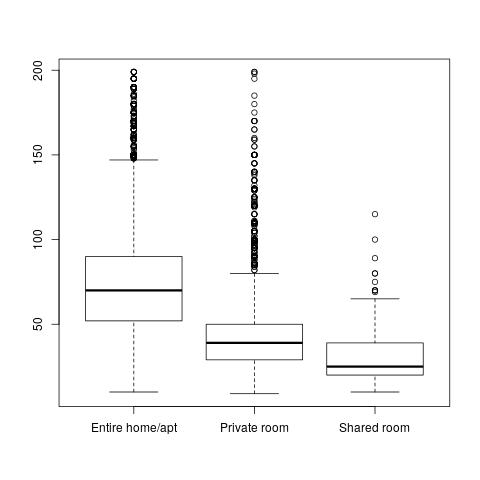
\includegraphics[width=0.35\textwidth]{boxplotPrijsCity.jpg}
	\end{center}
	\caption{Boxplot type vs prijs.}
	\label{fig:bpc}
\end{wrapfigure}
Een boxplot (\ref{fig:bpc}) zonder de extreme outliers lijkt te suggereren  dat er een verschil blijkt te zijn tussen de types, vooral tussen een volledig huis/appartement en de rest.
Om overzicht te behouden hebben we de bovenste outliers uit de figuur gelaten, waarvan er nog 705 tussen 150 en 1500 lagen en nog 8 hoger dan 1500 met een maximum van 8944. 
De prijs lijkt aan de hand van figuur \ref{fig:pv} (zonder outliers) een redelijke klokcurve voor te stellen met een zeer lichte linkerstaart en een erg zware rechterstaart. 
De prijs lijkt niet normaal verdeeld door outliers en de knik in de curve (qqplot \ref*{fig:qqp}). 
Een schatting van de lambda voor een Box-Cox transformatie raad -0.2549 (afgerond $-\frac{1}{4}$) aan als lambda.
Figuur \ref{fig:qqbp} toont een verbetering qua normaliteit.
Deze transformatie gaf de beste verbetering van alle geteste transformaties (log10, sqrt, log10(log10)).
\begin{figure}[H]
	\centering
	\begin{subfigure}[b]{0.23\textwidth}
		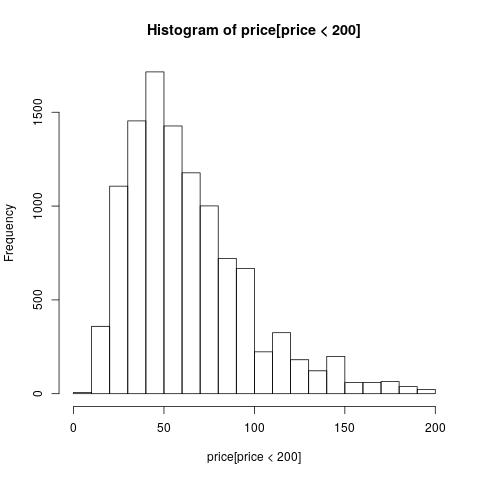
\includegraphics[width=\textwidth]{prijsVis.jpg}
		\caption{Visualisatie van de prijs.}
		\label{fig:pv}
	\end{subfigure}
	~ %add desired spacing between images, e. g. ~, \quad, \qquad, \hfill etc. 
	%(or a blank line to force the subfigure onto a new line)
	\begin{subfigure}[b]{0.23\textwidth}
		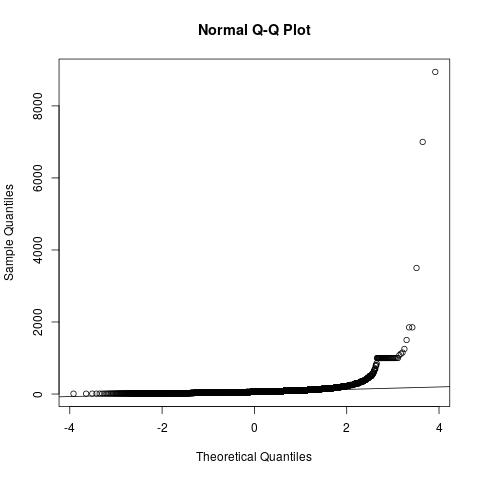
\includegraphics[width=\textwidth]{qqp.jpg}
		\caption{Kwantielplot prijs}
		\label{fig:qqp}
	\end{subfigure}
	~
	\begin{subfigure}[b]{0.23\textwidth}
		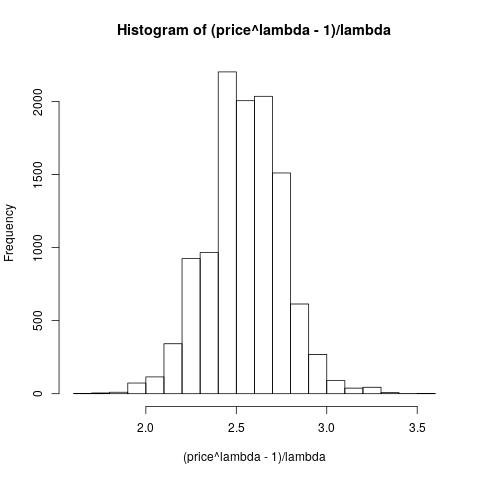
\includegraphics[width=\textwidth]{prijsB.jpg}
		\caption{Visualisatie Box-Cox  $-\frac{1}{4}$ prijs}
		\label{fig:bpv}
	\end{subfigure}
	~ %add desired spacing between images, e. g. ~, \quad, \qquad, \hfill etc. 
	%(or a blank line to force the subfigure onto a new line)
	\begin{subfigure}[b]{0.23\textwidth}
		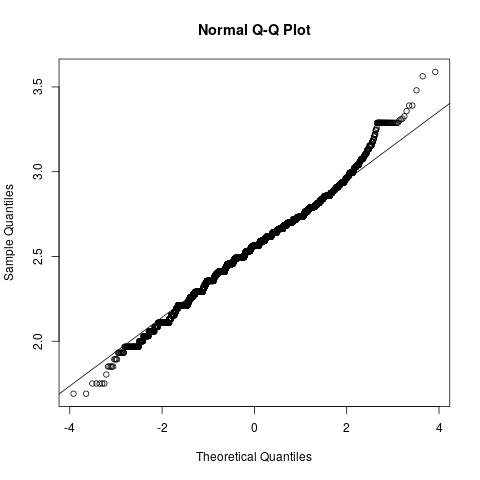
\includegraphics[width=\textwidth]{qqbp.jpg}
		\caption{Kwantielplot Box-Cox -1/4 prijs}
		\label{fig:qqbp}
	\end{subfigure}
\end{figure}


De Box-Cox transformatie komt er als beste uit als we residuals analyseren van een model met de verschillende transformaties (figuur \ref{fig:pcqq}).
We nemen voor de rest van deze sectie die transformatie voor de prijs.
De Levene test toont aan dat er heteroscedasticiteit is, wat aannemelijk lijkt gegeven figuur \ref{fig:bpc}.
Kwantielplot \ref{fig:pcqq} toont dat de residuals niet normaal verdeeld zijn.
Het aantal samples is te groot om een Shapiro test op uit te voeren.
Een plot tegenover de index \ref{fig:pcisr} toont geen afhankelijkheid ``in de tijd''.
Niet alle modelveronderstellingen voor de relevante testen zijn voldaan, onze bevindingen moeten daarom met een korrel zout genomen worden.\\
Het model verwierp de f-test en t-test voor alle variabelen. 
De R-squared en adjusted R-squared  waren echter maar 0.268.
De weighted least square methode toonde geen verbeteringen op het model na 1 iteratie. 
De aov methode (partiële F-test met Bonferroni correctie) toont alsook aan dat het type verblijf effectief significant is voor de prijs.
De tukey-test toont aan dat de verschillende soorten kamers onderling ook genoeg verschillen van elkaar. \\
Conclusie: het type verblijf is significant voor de prijs en de types verschillen onderling allemaal in prijs. Volgens de coëfficiënten van het model is de prijs als volgt gerangschikt: 
volledig huis app. > privé kamer > gedeelde kamer.
Deze bevindingen stroken met de vermoedens van de realiteit.

\begin{figure}[H]
	\centering
	\begin{subfigure}[b]{0.3\textwidth}
		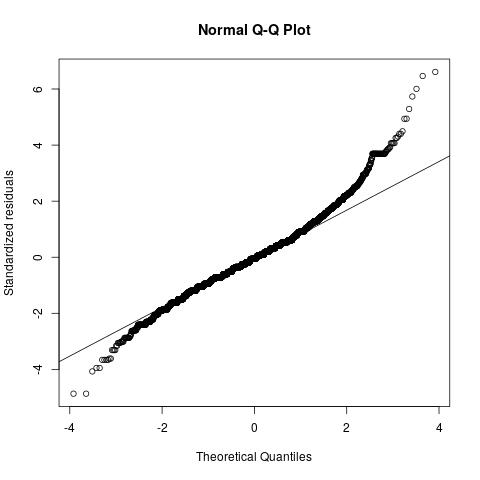
\includegraphics[width=\textwidth]{pcqq.jpeg}
		\caption{Kwantielplot gestandardiseerde residuals}
		\label{fig:pcqq}
	\end{subfigure}
	~ %add desired spacing between images, e. g. ~, \quad, \qquad, \hfill etc. 
	%(or a blank line to force the subfigure onto a new line)
	\begin{subfigure}[b]{0.3\textwidth}
		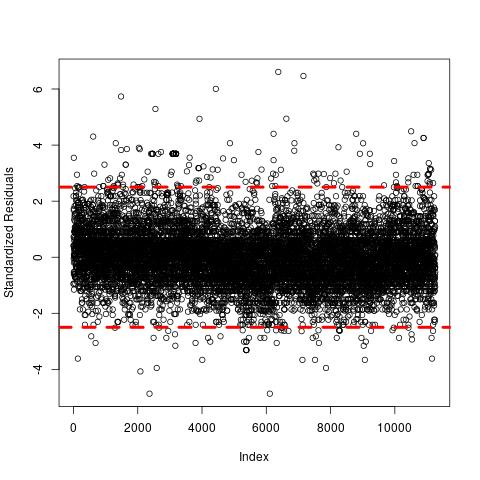
\includegraphics[width=\textwidth]{pcisr.jpeg}
		\caption{Index vs gest. residuals}
		\label{fig:pcisr}
	\end{subfigure}
\end{figure}

\subsection{stad vs huurprijs}
\label{sec:stadvsprijs}
De boxplot zonder outliers (figuur \ref{fig:bpcit}) suggereert  dat er niet veel verschil is in de gemiddelde prijs per stad. Antwerpen en Gent zijn nagenoeg het zelfde, enkel de prijzen in Brussel liggen wat lager. \\
We zien dat de residuals niet normaal verdeeld zijn (figuur \ref{fig:qqboxcit}), waardoor onze bevindingen opnieuw niet steenhard mogen genomen worden. De Levene test kan echter niet verwerpen dat er homoscedasticiteit.\\
Het model verwerpt de f-test en t-test voor de variabelen van Antwerpen (= het intercept) en Brussel, maar Gent is niet verworpen  met een p-waarde van 0.068. 
Antwerpen krijgt ``voorrang'' aangezien het het intercept is, en de gelijkenissen tussen Antwerpen en Gent uit figuur \ref*{fig:bpcit} dit kunnen verklaren. 
De reden dat Gent dus niet verworpen is, is omdat hij heel sterk op Antwerpen lijkt, wat dus betekent dat beiden niet significant verschillen qua prijs.
Het kleine verschil in de coëfficiënten bevestigd dat.
Aov zegt dat de stad significant is voor de prijs. 
De residuals zijn niet afhankelijk van de tijd/index (figuur \ref{fig:indc}).
De R-squared van dit model is 0.0226 en de adjusted is 0.0224, wat dus opnieuw niet goed is.
De Tukey-test verwerpt sterk dat er geen verschil zou zijn tussen Brussel en de andere twee steden. Maar Gent en Antwerpen worden niet verworpen  met een p-waarde van 0.162, wat opnieuw onze vermoedens bevestigd. 
Het effect van Brussel is ook veel sterker dan die van Antwerpen en Gent. 
Conclusie: de stad is significant voor de prijs. Er is een prijsverschil tussen Brussel en de andere 2 steden, maar er is geen significant prijsverschil tussen Antwerpen en Gent.
De coëfficiënten van het model vertellen dat Brussel goedkoper is dan de andere 2 steden, wat strookt met de boxplot op figuur \ref{fig:bpcit}.

\begin{figure}[H]
	\centering
	\begin{subfigure}[b]{0.3\textwidth}
		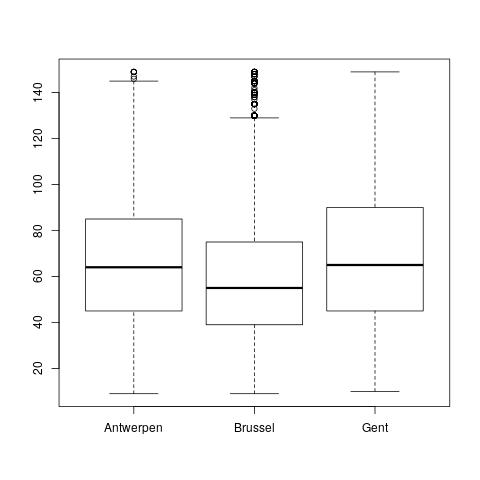
\includegraphics[width=\textwidth]{boxprijscity.jpg}
		\caption{Boxplot stad vs prijs.}
		\label{fig:bpcit}
	\end{subfigure}
	~ %add desired spacing between images, e. g. ~, \quad, \qquad, \hfill etc. 
	%(or a blank line to force the subfigure onto a new line)
	\begin{subfigure}[b]{0.3\textwidth}
		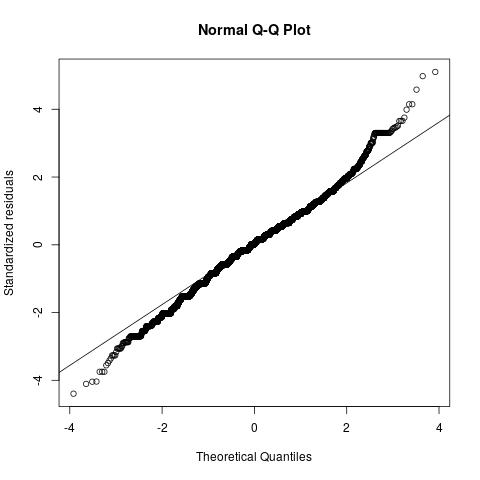
\includegraphics[width=\textwidth]{qqboxcit.jpg}
		\caption{QQplot gestandaardiseerde residuals model}
		\label{fig:qqboxcit}
	\end{subfigure}
	~
	\begin{subfigure}[b]{0.3\textwidth}
		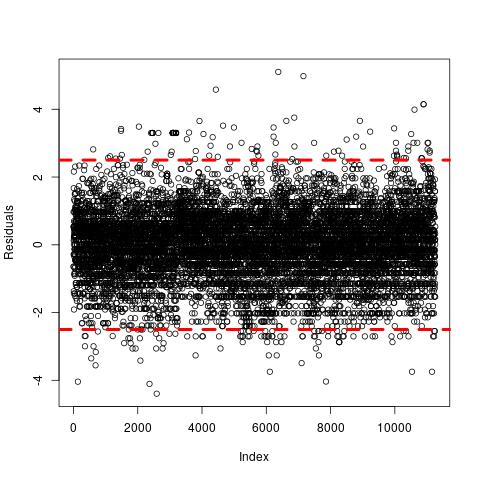
\includegraphics[width=\textwidth]{indc.jpg}
		\caption{Index vs residuals}
		\label{fig:indc}
	\end{subfigure}
\end{figure}

\subsection{Buurten}
Op het eerste zicht (figuur \ref{fig:boxne}) lijken de buurten niet zo veel te verschillen.
Het model waarbij we enkel neighbourhood meenemen, verwerpt de f-test, maar een groot deel van de neighbourhoods worden niet verworpen door de t-test (43/96). 
De Levene test en een normale qqplot tonen dat er heteroscedasticiteit is en de residuals niet normaal zijn,dus onze bevindingen moeten daarom met een korrel zout genomen worden.
Residual zijn niet afhankelijk van de tijd/index (figuur \ref{fig:stdne})
Aov toont aan dat de buurt significant.
De TukeyTest verteld dat 47,6\% van de combinaties van buurten  niet significant verschillen.
De R-squared is 0.099 en adjusted 0.091, wat opnieuw aan de lage kant is.
Alleen lijkt dus dat de buurt significant is in het algemeen, maar zeer veel buurten onderling te weinig verschillen.
Dit doet suggereren dat de opdeling per buurt te verfijnt is.


\begin{figure}[H]
	\centering
	\begin{subfigure}[b]{0.3\textwidth}
		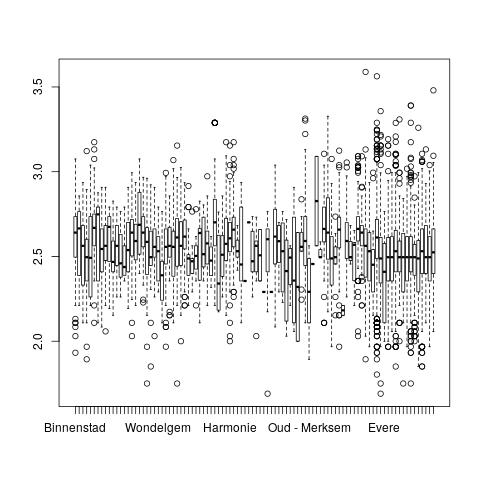
\includegraphics[width=\textwidth]{boxne.jpg}
		\caption{Boxplot buurt vs prijs.}
		\label{fig:boxne}
	\end{subfigure}
	~ %add desired spacing between images, e. g. ~, \quad, \qquad, \hfill etc. 
	%(or a blank line to force the subfigure onto a new line)
	\begin{subfigure}[b]{0.3\textwidth}
		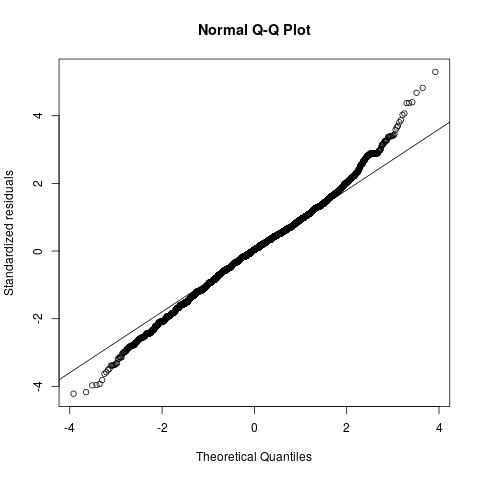
\includegraphics[width=\textwidth]{qqne.jpg}
		\caption{QQplot gestandaardiseerde residuals model}
		\label{fig:qqne}
	\end{subfigure}
	~
	\begin{subfigure}[b]{0.3\textwidth}
		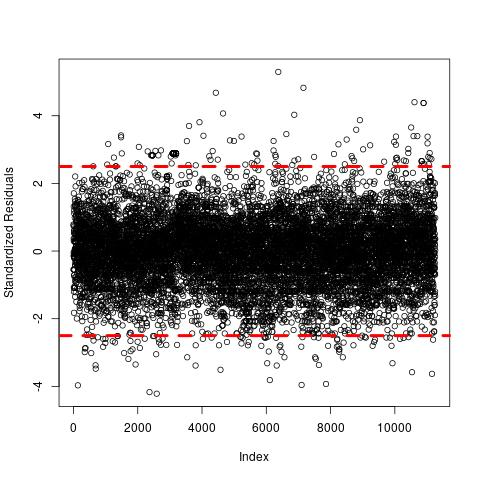
\includegraphics[width=\textwidth]{stdne.jpg}
		\caption{Index vs residuals}
		\label{fig:stdne}
	\end{subfigure}
\end{figure}

\subsection{Buurten en stad}
Het model met de buurt en de stad verwerpt de f-test ook met, maar een nog groter deel van  wordt niet verworpen door de t-test (54). Meer bepaald is de pwaarde van Gent zeer hoog (0.9) terwijl Antwerpen en Brussel nog steeds verworpen worden. 
De R-squared is 0.099 en adjusted 0.091 (onveranderd). Dit doet vermoeden dat beide dus sterk verbonden zijn aangezien hun gecombineerd model even slecht is als hun afzonderlijke.
Aov verwerpt echter voor beide variabelen.
De Tukey test kan nu nog 44,6\% van de combinaties verwerpen.
Deze bevindingen suggereren dat door de buurt en de stad beiden op te nemen, de significantie van Gent vs. Antwerpen miniem wordt. De Aov verwerpt niet dat een van de twee overbodig wordt, maar aangezien zeer veel variabelen de t-test falen, er geen verbetering is in de R-squared en het nog steeds hoge percentage van het niet verwerpen van de Tukey test tonen dat het origineel probleem van het te verfijnd zijn van de buurtenverdeling enkel nog maar versterkt wordt door de stad erbij te nemen.



\begin{figure}[H]
	\centering
	\begin{subfigure}[b]{0.3\textwidth}
		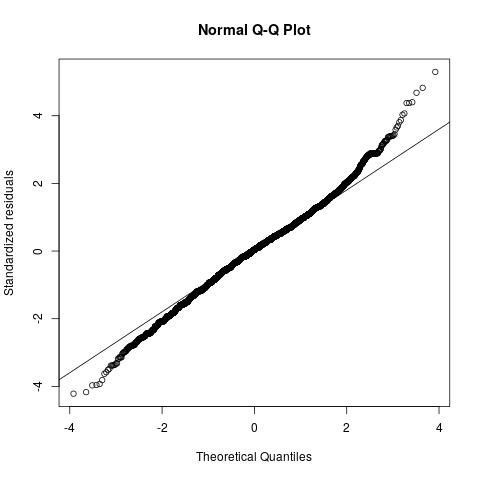
\includegraphics[width=\textwidth]{qqnes.jpg}
		\caption{QQplot gestandaardiseerde residuals model}
		\label{fig:qqnes}
	\end{subfigure}
	~
	\begin{subfigure}[b]{0.3\textwidth}
		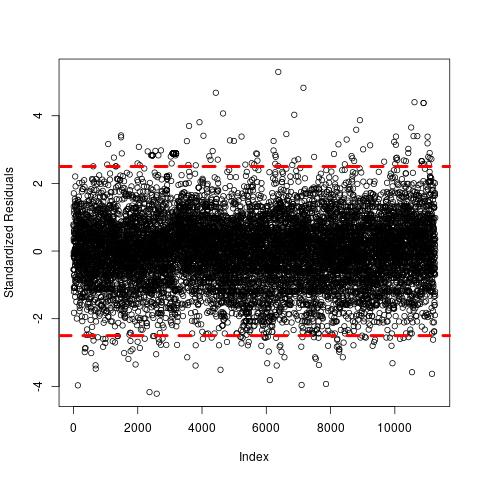
\includegraphics[width=\textwidth]{stdnes.jpg}
		\caption{Index vs residuals}
		\label{fig:stdnes}
	\end{subfigure}
\end{figure}
\begin{wrapfigure}{r}{0.4\textwidth}
	\begin{center}
		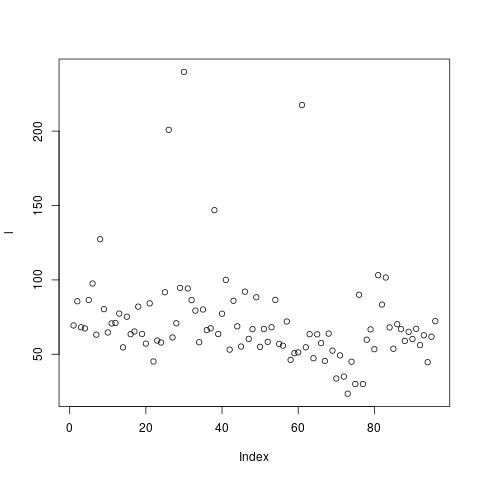
\includegraphics[width=0.35\textwidth]{pn.jpg}
	\end{center}
	\caption{Gemiddelde prijs per buurt.}
	\label{fig:pn}
\end{wrapfigure}
Figuur \ref{fig:pn} toont dat er een ongeveer 5 buurten zijn die een opvallend hogere prijs hebben dan de rest.
De gemiddelde huurprijs is 72,2 euro.
Woluwe-Saint-Pierre steekt hier sterk boven met een gemiddelde huurprijs van 240 euro.
Daarna volgt Sint Denijs Westrem met 217,5 en Oud-Berchem met 201.
Deze drie zijn significant hoger dan de rest in liggen in Brussel, Gent en Antwerpen. Niet in een bepaalde stad dus.
Dan zijn er nog 2 minder extreem prijzige gemeenten, namelijk Eilandje met 147 en Polder met 127 (beiden liggen in Antwerpen). De eerste opeenvolgende is nog maar 103.
Daarnaast zijn er nog 5 Antwerpse buurten waar de prijs ietwat lager ligt dan de rest met prijzen tussen 23,5 en 35 euro.
Deze zijn echter minder een stuk minder ver verwijdert van het gemiddelde in vergelijking met de extreem prijzige outliers.

\subsection{Buurten en type verblijf}
Opnieuw werd de f-test verworpen en 42 t-testen faalden.
Aov verwerpt echter voor beide variabelen.
De R-squared is sterk gestegen van 0.099 naar 0.3281 en de adjusted van 0.091 naar 0.3222.
De R-squared van room-type alleen was ook 0.2678 en de adjusted 0.2677. De combinatie van de 2 variabelen versterken elkaar dus.
De buurt en het type verblijf maken elkaar dus niet overbodig.




\section{Model voor de huurprijs} \label{sec:mh}
Op basis van relevante beschikbare gegevens hebben we geprobeerd een model op te stellen om de prijs van een Airbnb-verblijf zo goed mogelijk te voorspellen. Eerst moesten we daarvoor kijken welke gegevens er relevant zouden zijn voor ons model. Daarna controleerden we of het nodig was om bij bepaalde variabelen een transformatie toe te passen. We bekeken enkele modellen met en zonder transformaties en tot slot bepaalden we het beste model om de prijs te voorspellen.
\subsection{Selectie relevante gegevens}
\label{sec:huurprijsSelectie}
Voor we beginnen met een model te zoeken verwijderen we alle rijen die een kolom missen. Het aantal samples gaat dan van 11262 naar 9476.\\

Om variabelen te selecteren als een relevante variabele voor ons model, keken we naar hoe de prijs zich verhoudt ten opzichte van de variabele. We laten de naam en id van het verblijf en van de host achterwege omdat id willekeurig zijn voor de andere attributen van een zoekertje.
De naam (of id) van het verblijf is zinloos omdat dit een 1 op 1 relatie is per zoekertje en dit dus gigantische overfitting zou zijn.
De naam van de host (of hun categorische id) zou in principe kunnen meegenomen worden, maar dit doen we niet om 3 redenen:
\begin{itemize}
	\item kan gezien worden als sterke overfitting (zie puntje 3)
	\item het model wordt op die manier onoverzichtelijk 
	\item het model heeft op die manier geen enkele betekenis meer als een nieuw verhuurder op de site komt en heeft dus geen voorspellende kracht om te voorspellen. 
\end{itemize} 

De variabele "'latitude"' blijkt wel een in vloed te hebben op de prijs. Als we kijken naar de waarden van de breedtegraden dan zien we dat we deze kunnen indelen in de drie steden. We gaan in plaats van de breedtegraad in ons model te gebruiken, gebruik maken van de variabele "'city"'. "'Longitude"' wordt om dezelfde reden niet gebruikt in het model, deze variabele deelt de data op in twee delen namelijk als eerste deel Gent en als tweede deel Brussel en Antwerpen. Vervolgens zien we ook dat variabelen "'room\_type"', "'minimum\_nights"', "'number\_of\_reviews"', "'last\_review"', "'reviews\_per\_month"', "'availability\_365"' en "'calculated\_host\_listings\_count"' relevant kunnen zijn voor ons model. \\

Voor de variabelen die iets zeggen over de reviews hebben ook eens gekeken naar de correlatie tussen deze variabelen. We vonden dat er een sterke correlatie bestaat tussen "'reviews\_per\_month"' en "'number\_of\_reviews"', ook is er een correlatie tussen "'reviews\_per\_month"' en "'last\_review"'. Om deze reden gaan we zeker al twee verschillende modellen opstellen waarbij enerzijds gewerkt wordt met alle drie de variabelen en anderzijds enkel met de variabele "'reviews\_per\_month"'.\\

In tabel \ref{tab:transformaties} is een samenvatting te zien van de relevante gegevens die we zullen gebruiken voor ons model op te stellen.
\begin{table}[!h]
	\centering
	\begin{tabular}{|l|l|l|}
		\hline 
		\textbf{Variabele} & \textbf{Afkorting}& \textbf{Transformatie} \\ 
		\hline 
		room\_type & $R_{private}$, $R_{shared}$,$R_{entire}$&/ \\ 
		%\hline 
		city & $C_{Gent}$, $C_{Antw}$,$C_{Brussel}$&/ \\ 
		%\hline 
		price & $P$&$\frac{(P^{(-0.25)}) - 1}{-0.25}$ \\ 
		%\hline 
		minimum\_nights & $MN$&$\frac{(MN^{(-0.67)}) - 1}{-0.67}$ \\ 
		%\hline 
		number\_of\_reviews & $NbRev$& $log_{10}(NbRev)$\\ 
		%\hline 
		last\_review & $LRev$&$ log_{10}(LRev + 1) $\\
		%\hline
		reviews\_per\_month &$RevMonth$&$ log_{10}(RevMonth) $ \\
		%\hline
		calculated\_host\_listings\_count &$CHLC$& $\frac{(CHLC^{(-1)}) - 1}{-1}$\\
		%\hline
		availability\_365 & $Av$&/\\ \hline
	\end{tabular} 
	\caption{Samenvatting van de relevante variabelen en hun transformaties.}
	\label{tab:transformaties}
\end{table}
\subsection{Transformaties}
In deze sectie bekijken we of er transformaties zijn die ervoor kunnen zorgen dat we een beter model verkrijgen om de prijs te voorspellen. Het spreekt voor zich dat we hier enkel naar de numerieke variabelen kijken. In tabel \ref{tab:transformaties} is een samenvatting te zien van de gevonden transformaties. Voor elke variabele vergeleken we de identieke met een log10 en Box-Cox transformatie. Hiervoor werd gekeken naar de boxplot, normale kwantielplot en het histogram. In figuur \ref{fig:transformVb} is een voorbeeld te zien van hoe we te werk gingen, de variabele hier is het aantal reviews per maand. De bovenste drie figuren zijn van de identieke, voor de onderste drie is de log10 transformatie toegepast. Het is duidelijk dat de log10 transformatie voor het aantal reviews per maand hier een verbetering geeft.

\begin{figure}[H]
	\centering
	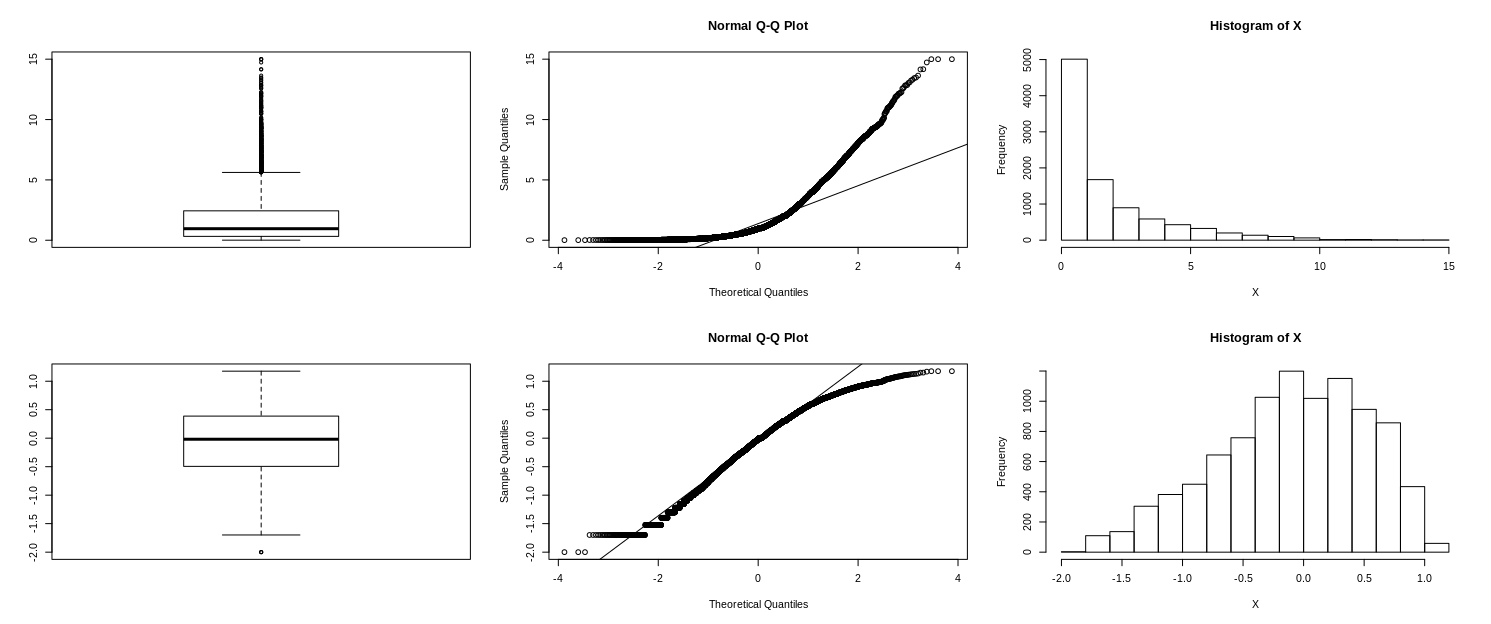
\includegraphics[width=\textwidth]{transformatieVb.jpeg}
	\caption{Voorbeeld van een verbetering door log10 transformatie op het aantal reviews per maand. Eerste drie grafieken zijn de boxplot, normale kwantielplot en het histogram zonder transformatie, de andere drie zijn de grafieken van de log10 transformatie.}
	\label{fig:transformVb}
\end{figure}

\subsection{Modellen}
Om een goed model te vinden zijn we als volgt te werk gegaan: ons eerste model ontstond van uit alle relevante niet-getransformeerde variabelen het beste model te nemen. Met een R-squared van 0.032 vonden we dit model zeer slecht en dus gingen we verder naar het model met de getransformeerde variabelen. Hierbij merkten we direct een grote verbetering in de R-squared (= 0.37). In het derde en vierde model dat we bekeken, lieten we de variabelen laatste review en aantal reviews weg. Hier keken we weer naar de modellen met niet-getransformeerde en getransformeerde variabelen. Het derde model bleek gelijk te zijn aan het eerste model, dit is te verklaren omdat bij het opstellen van het eerste model de twee review variabelen uiteindelijk ook weggelaten werden. Tot slot hebben we nog het vierde model, dit model is zo goed als gelijk aan het tweede model met het enige verschil dat de getransformeerde variabele laatste review hier niet in meegenomen is. \\

Voor de twee beste modellen van hierboven hebben we ook gekeken of er een verbetering was als we met interactietermen werkten. Hierbij zagen we dat die modellen niet beter waren dan de modellen die we al hadden. Bij het kijken naar de multicollineariteit van de modellen zonder en met interactietermen, zagen we dat die zonder interactietermen een veel kleinere multicollineariteit hadden dan die met interactietermen. Hieruit concluderen we dus dat het tweede en vierde model van hierboven beter zijn. \\

Aangezien het tweede en vierde model enkel verschilde in het al dan niet opnemen van de getransformeerde variabele laatste review, keken we ook eens naar hoe significant de bijdrage was van deze variabele. Hieruit bleek dat deze bijdrage niet significant was en besluiten we dat het vierde model het beste was. De co\"effici\"enten van beide modellen zijn ook zo goed als gelijk.\\

We weten dat de prijsvariabele extreme outliers heeft, dit is dan ook de verklaring waarom de twee modellen zonder getransformeerde variabelen zeer slecht waren. Als we keken naar het eerste en vierde model die niet be\"invloed werden door de outliers, dan bleek dat het eerste model ongeveer een even goede voorspelling geeft voor de prijs als het vierde model (respectievelijk is de R-squared 0.45 en 0.43). Voor het vierde model zonder outliers was er niet zo'n groot verschil te merken in de co\"effici\"enten met het initi\"ele vierde model, dit komt omdat door de transformatie er al veel outliers onderdrukt zijn.\\
%TODO: checken op multicolllineariteit (bvb gent en antwerpen)
% en bespreken van de modelproblemen. bvb outliers zijn bad leverage points en doe een diagnostic plot (p337)
\subsection{Conclusie}
We concluderen dat het eerste model het beste model is als de outliers onderdrukt worden. Dit is het gevonden model:
\begin{multline}
price = 62.18 - 26.05\cdot R_{private}  - 44.06\cdot R_{shared}  - 0.30\cdot RevMonth + \\1.09\cdot CHLC + 0.025 \cdot Av - 3.04\cdot C_{Brussel} + 6.04\cdot C_{Gent}
\end{multline}
Eerst en vooral zien we hier dat de gemiddelde prijs voor het huren van een volledig huis/appartement, in Antwerpen, die altijd verhuurd is, geen reviews per maand heeft en de uitbater maar 1 verblijf heeft, ongeveer \euro  63.27 bedraagd. Daarnaast daalt de voorspelling van de prijs een stuk als er sprake is van een priv\'e of gedeelde kamer. Zoals we in sectie \ref{sec:stadvsprijs} al zagen, is hier ook duidelijk dat de prijzen in Gent iets hoger liggen dan in Antwerpen en dat de prijzen in Brussel lager zijn dan in Antwerpen en Gent.\\

De andere drie variabelen hebben minder significante co\"effici\"enten. We kunnen afleiden uit dit model dat het aantal verblijven van de uitbater een kleine rol speelt in het voorspellen van de prijs. 
\textbf{Het volgende mag je niet zeggen, omdat er correlatie is tussen de x'en, herrinner je van stat 1, ik doe dit omdat hij het zelf zo zegt van die kansen, maar van een gewoon regressiemodel mag je dat niet zeggen}
Ook merken we dat er elke de 40 dagen dat het verblijf niet verhuurd wordt, de prijs een euro stijgt. 

\section{Beschikbaarheid van een verblijf}
In deze sectie proberen we logistische regressie toe te passen om te voorspellen of een verblijf al dan niet wordt vast verhuurd in plaats van enkel voor korte periodes.
We proberen een model te vinden, dit te evalueren en te interpreteren.
\subsection{Model selectie}
De proporties van categorische veranderlijken worden hierdoor niet significant aangepast.
Het aantal beschikbare dagen wordt natuurlijk niet opgenomen als regressor omdat het al dan niet permanent verhuurd zijn direct hieruit is afgeleid. Ook hier laten we de id's en namen achterwege.


We pasten AIC gebaseerde voorwaartse, achterwaartse en stapsgewijze regressie toe.
Dit deden we 2 maal, de 2e keer met de variabelen in de omgekeerde volgorde.
Hierbij werden de prijs, het type, het minimum aantal nachten, het aantal zoekertjes per host, de datum van de laatste review, het aantal reviews per maand en het aantal reviews van het afgelopen jaar telkens geselecteerd.
De buurt werd nooit geselecteerd, de stad 2 keer en de latitude en longitude 4 keer. Stad werd enkel geselecteerd als latitude en longitude niet geselecteerd werden en omgekeerd, wat dus suggereert dat ze dezelfde informatie toevoegen aan het model, wat ook strookt met de realiteit van de soort variabelen (zie sectie \ref{sec:huurprijsSelectie}).
Stad is de nette classificatie van latitude en longitude, daarom vergelijken we een model met latitude en longitude tegenover een model met de stad in de plaats.
De buurt laten we achterwege.
De bekomen modellen hebben dezelfde AIC en deviance waarden en resulteren in hetzelfde voor de likelihood ratio test en de goodness of fit test, behalve dat latitude maar zwak verworpen wordt in hun eigen model.
Omdat de stad de significantie van latitude en longitude mooi samenvat gaan we verder met de stad en laten we latitude en longitude vallen.  
% kga het laten staan omdat het over een andere variabele gaat, ma je hebt wel gelijk, ma tstaat er nu en de sectie over vraag 3 is niet lang
In de testen wordt echter niet verworpen dat het type er niet toe doet.
Omdat deze echter altijd in de geselecteerde modellen zat en het bijna verworpen was nemen we het toch mee in ons model.
Omdat normaliteit van de regressoren de kwaliteit van een model sterk beinvloeden gebruiken we dezelfde transformaties als in sectie \ref{sec:mh}.
Voor de interpretatie hanteren we echter een model zonder transformaties om ons meer zinvol te kunnen uitspreken over het model. 
\subsection{Model evaluatie}

De Wald test verwerpt het niet significant zijn van de enkele variabelen allemaal  met voldoende marge.
De behaalde deviance is 6305.7 en de AIC 6327.7.
Dit is een daling van ongeveer 1000 tegenover het model zonder transformaties.
\begin{wrapfigure}{r}{0.4\textwidth}
	\begin{center}
		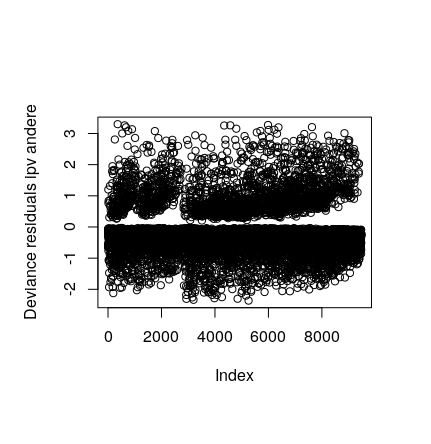
\includegraphics[width=0.35\textwidth]{Rplot.png}
	\end{center}
	\caption{Deviance residuals.}
	\label{fig:rpn}
\end{wrapfigure}
De likelihood ratio test verwerpt ook voor alle regressoren dat ze niet significant zouden zijn met voldoende marge.
De deviance residuals (figuur \ref{fig:rpn}) vertonen niets zorgbarends, behalve dat er een opslitsing te zien is tussen de steden, mede veroorzaakt omdat ze aan elkaar geplakt zijn en dus gegroepeerd in de data.
De goodness of fit test verwerpt ook sterk.
Qua problemen is er de duidelijke opsplitsing van de deviance residuals, maar de oorzaak is bekend en geeft geen verdere problemen.
Doordat de residuals niet normaal verdeeld zijn bij logistische regressie kan er ook niet sterk gecontroleerd worden op problemen met normaliteit of modelveronderstelling om problemen te vinden.
\subsection{Model interpretatie}
Het model met dezelfde variabelen maar ongetransformeerd kan als volgt geïnterpreteerd worden:\\
\textit{Als hier gezegd wordt meer kans, wordt veronderstelt dat alle andere variabelen strikt onveranderd blijven en gegeven zijn.}\\
Iemand in Brussel heeft 54 procent meer kans dat het vol zit dan in Antwerpen. Iemand in Gent   73\% meer kans dat het vol zit dan in Antwerpen.
Iemand die een privé kamer zoekt heeft 22.5 procent meer kans dat het vol zit dan bij een volledig huis of appartement.
Iemand die een gedeelde kamer zoekt   heeft 16.2 procent minder kans dat het vol zit dan bij een  volledig huis of appartement.
Je hebt meer kans dat het verblijf permanent verhuurd is als:
\begin{itemize}
	\item prijs -     (1.2)
	\item laatste review  + (0.3)
	\item aantal reviews - (0.7)
	\item reviews maand - (22.1)
	\item minimum nachten - (3)
	\item zoekertjes uitbater - (4)
\end{itemize}
waarbij -/+ betekent de kans stijgt als het attribuut daalt/stijgt.
Het cijfer tussen de haakjes is het percentage dat de kans stijgt of daalt bij het veranderen van 1 van het attribuut.
Als het langer geleden is dat de laatste review werd geschreven heb je een grotere kans dat het verblijf permanent verhuurd is.
Als de prijs, het aantal reviews in totaal en per maand, het minimum aantal nachten en het aantal zoekertjes per uitbater lager is, heb je een grotere kans dat het verblijf permanent verhuurd is.
Dit strookt met wat je zou denken dat er in de realiteit gebeurt, behalve dan het minimum aantal nachten.
Mogelijks is dit omdat je maximum aantal minimum nachten 30 dagen kan zijn en dus niet relevant is voor permanente huurders, waardoor ze het gewoon op 1 laten staan.


\end{document}
